%\RequirePackage[l2tabu, orthodox]{nag}
\documentclass[12pt,a4paper,headinclude]{scrartcl}

\usepackage[utf8]{inputenc}

\usepackage{latexsym,exscale,amssymb,amsmath}
%\usepackage{paralist}
\usepackage{algorithm}
\usepackage{algpseudocode}
%\usepackage[colorinlistoftodos]{todonotes}
\usepackage{xspace}
\usepackage{array}
\usepackage{amsfonts}
\usepackage{graphicx}
\usepackage{siunitx}
\usepackage{microtype}
\usepackage{url}
\usepackage{hyperref}
\usepackage{subcaption}
\usepackage{multirow}
%\usepackage[margin=0.8in, tmargin=0.5in]{geometry}

\usepackage[
backend=biber,	
%    style=authoryear-icomp,
%    sortlocale=de_DE,
%    natbib=true,
url=false, 
doi=true,
eprint=false,
isbn=false,
sorting=none
]{biblatex}
\addbibresource{Neuroscience.bib}


\newcommand{\corresponds}{\ensuremath{\mathrel{\widehat{=}}}}
\newcommand{\pd}[2] {\frac{\partial #1}{\partial #2}}
\newcommand{\pdsqu}[2] {\frac{\partial^2 #1}{\partial #2^2}}
%\newcommand{\diff}[2] {\frac{\text{d} #1}{\text{d} #2}}
\newcommand*\diff{\mathop{}\!\mathrm{d}}
\newcommand*\Diff[1]{\mathop{}\!\mathrm{d^#1}}
%\newcommand{\d}[0] {\text{d}}
\newcommand{\celsius}{$^\circ$ C}

\newcommand{\Tv}{\textsc{Tv}\xspace}
\newcommand{\bigO}{\mathcal{O}}
\newcommand{\latex}{\LaTeX\xspace}
\newcommand{\pdf}{\textsc{Pdf}\xspace}
\newcommand{\ordo}{\mathcal{O}}
\newcommand{\mset}[1]{\lbrace #1 \rbrace}

%makes column vectors: \colvec{5}{a}{b}{c}{d}{e}
\newcount\colveccount
\newcommand*\colvec[1]{
        \global\colveccount#1
        \begin{pmatrix}
        \colvecnext
}
\def\colvecnext#1{
        #1
        \global\advance\colveccount-1
        \ifnum\colveccount>0
                \\
                \expandafter\colvecnext
        \else
                \end{pmatrix}
        \fi
}

%%%%%%%%For Python listing%%%%%%%%%%%
% Default fixed font does not support bold face
\DeclareFixedFont{\ttb}{T1}{txtt}{bx}{n}{12} % for bold
\DeclareFixedFont{\ttm}{T1}{txtt}{m}{n}{12}  % for normal

% Custom colors
\usepackage{color}
\definecolor{deepblue}{rgb}{0,0,0.5}
\definecolor{deepred}{rgb}{0.6,0,0}
\definecolor{deepgreen}{rgb}{0,0.5,0}

\usepackage{listings}

% Python style for highlighting
\newcommand\pythonstyle{\lstset{
language=Python,
basicstyle=\ttm\small,
otherkeywords={self},             % Add keywords here
keywordstyle=\ttb\color{deepblue},
emph={MyClass,__init__},          % Custom highlighting
emphstyle=\ttb\color{deepred},    % Custom highlighting style
stringstyle=\color{deepgreen},
frame=single,                         % Any extra options here
showstringspaces=false,            % 
breaklines = True,
numbers = left
}}


% Python environment
\lstnewenvironment{python}[1][]
{
\pythonstyle
\lstset{#1}
}
{}

% Python for external files
\newcommand\pythonexternal[2][]{{
\pythonstyle
\lstinputlisting[#1]{#2}}}

% Python for inline
\newcommand\pythoninline[1]{{\pythonstyle\lstinline!#1!}}
%%%%%%%%%%%%%%%%%%%%%%%%%%%%%%


\begin{document}

\title{Estimating Intrinsic Timescales from Calcium Imaging}
%\subtitle{Assignment 1}
\date{\today}
\author{Jonas Dehning}

\maketitle

%\section{Correlation between non-moving electrode recordings}

\section{Introduction}

Calcium imaging has a range of advantages compared to electrode recordings, mainly that one can record a significantly larger number of individual neurons. The goal is to estimate the intrinsic timescale from the fluorescence traces obtained from two photon calcium imaging. The difficulty is that the decay time of the the widely used GCaMP6s calcium indicator is on the order of \SI{1.25}{s} to \SI{1.5}{s} and the intrinsic timescale is on the order of \SI{60}{} to \SI{200}{ms}. Furthermore, values of the autocorrelation function of the decay of the calcium indicator are  little smaller than 1, whereas we know from electrode measurement that the values of the autocorrelation function due to the intrinsic timescale are about 0.1. It is therefore completely hidden by the larger magnitude of the decay of the indicator.

The approach we want to take is to deconvolve the fluorescence signal in order to retrieve the spike times. From the spike times one can then calculate the autocorrelation function which is then hopefully determined by the intrinsic timescale. But one would like to test that this approach leads to the correct results.

There exists free datasets where neurons were recorded simultaneously with both calcium imaging and electrodes \cite{chen_ultrasensitive_2013,theis_benchmarking_2016}. From the electrode recordings precise spike times have been extracted. These datasets are therefore ideally suited to compare the autocorrelation functions obtained from the calcium traces to the ones obtained directly from the spike times.

\section{Methods}

The data that I used has been published as part of a challenge to build the best deconvolution algorithm for calcium imaging traces \cite{noauthor_spikefinder_nodate, theis_benchmarking_2016}. It has already been  preprocessed: for every neuron it contains the fluorescence trace with the neuropil contamination removed. It was then upsampled to \SI{100}{Hz} and the spikes binned with \SI{100}{Hz}. I analyzed the 3 recorded sessions where GCaMP6s was used as an indicator. Two sessions were recorded by Theis at al. \cite{theis_benchmarking_2016} and one by Chen et al. which first introduced this indicator \cite{chen_ultrasensitive_2013}. All were recorded in the primary visual cortex of mice with 10 to 20 neurons recorded simultaneously.

To deconvolve the fluorescence trace, I used the OASIS algorithm \cite{friedrich_fast_2017}. It is a very simple (15 lines of python code) online algorithm which considers the decay of the calcium indicator as an autoregressive process. Nevertheless it has a similar performance to other more complex algorithms \cite{pachitariu_robustness_2018}. As a part of the Suite2p toolbox \cite{pachitariu_suite2p:_2017} the usage is very straightforward. The only hyperparameter needed is the the decay time of the calcium indicator, which I set to \SI{1.5}{s}. 

To estimate the autocorrelation function, I averaged the autocorrelation function of all the neurons which were recorded in the session in order to reduce the noise. 

\section{Results}

The decay of the autocorrelation function obtained from deconvolution of calcium traces matches very well obtained from the spikes times of the electrode recordings. However, the first striking observation was that the values of the autocorrelation function from the deconvolved calcium traces are systematically larger than the one from the electrode recordings (Fig.~\ref{fig:comparison_2p}). I therefore normed the two autocorrelation to obtain similar amplitudes (Fig.~\ref{fig:comparison_2p_normed}). I was then positively surprised that the two functions match very well, especially the session recorded by Chen et al. (lower panel). The fast oscillations in the upper two panels could result from the upsampling of the calcium signal, which was done during preprocessing. 



\begin{figure}
\begin{subfigure}{.5\textwidth}
  \centering
  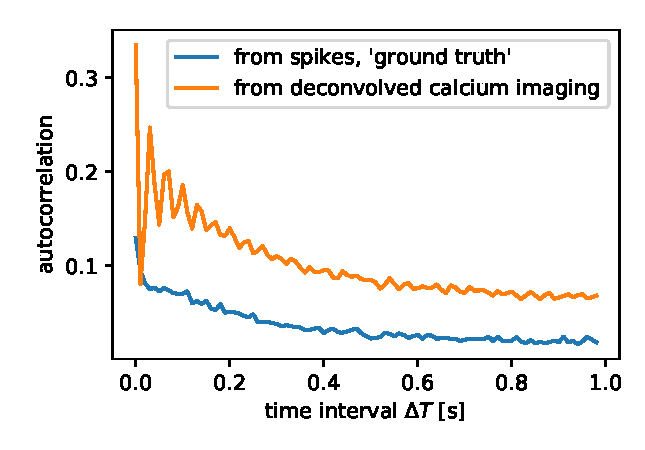
\includegraphics[width=1\linewidth]{./figures/comparison1.pdf}
\end{subfigure}%
\begin{subfigure}{.5\textwidth}
  \centering
  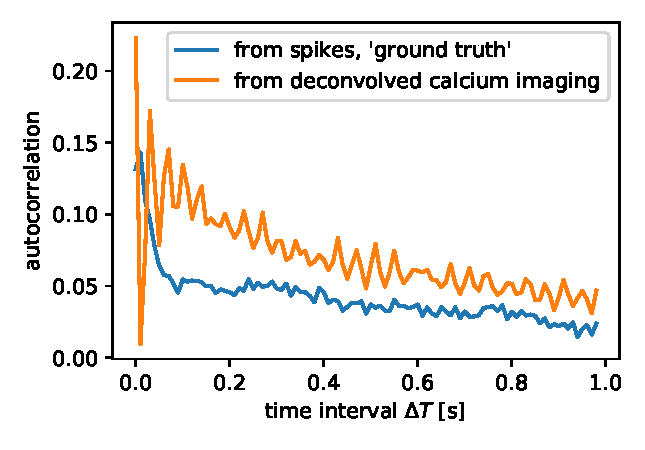
\includegraphics[width=1\linewidth]{./figures/comparison2.pdf}
\end{subfigure}%

\begin{subfigure}{1\textwidth}
	\centering
	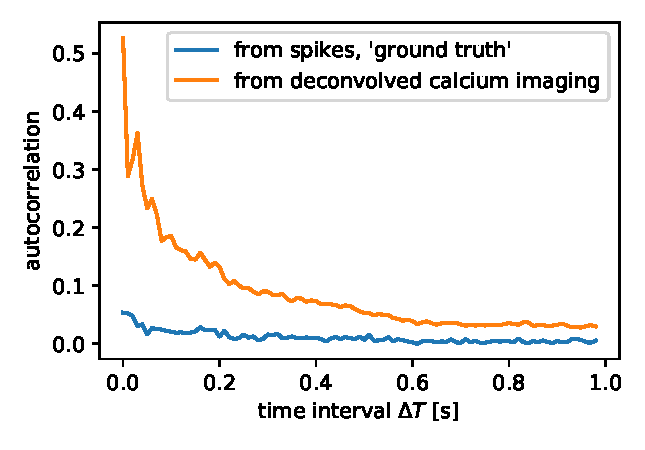
\includegraphics[width=0.5\linewidth]{./figures/comparison3.pdf}
\end{subfigure}%
\caption{The deconvolution approach tested against the autocorrelation function from electrophysiological spike recordings. The upper two figures of data from Theis et al. \cite{theis_benchmarking_2016}, the lower one from Chen et al. \cite{chen_ultrasensitive_2013}. The cause for the larger amplitude of the autocorrelation function from the calcium imaging is unknown.}
\label{fig:comparison_2p}
\end{figure}

\begin{figure}
	\begin{subfigure}{.5\textwidth}
		\centering
		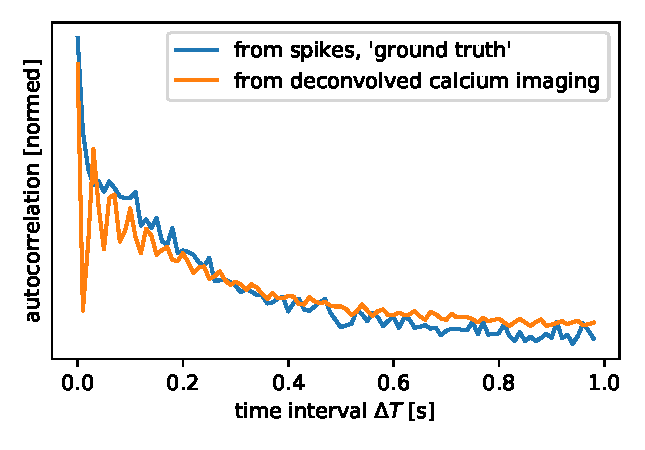
\includegraphics[width=1\linewidth]{./figures/comparison1_normed.pdf}
	\end{subfigure}%
	\begin{subfigure}{.5\textwidth}
		\centering
		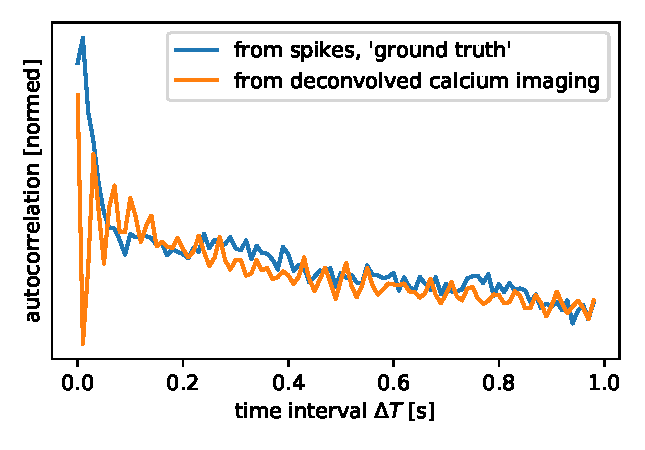
\includegraphics[width=1\linewidth]{./figures/comparison2_normed.pdf}
	\end{subfigure}%
	
	\begin{subfigure}{1\textwidth}
		\centering
		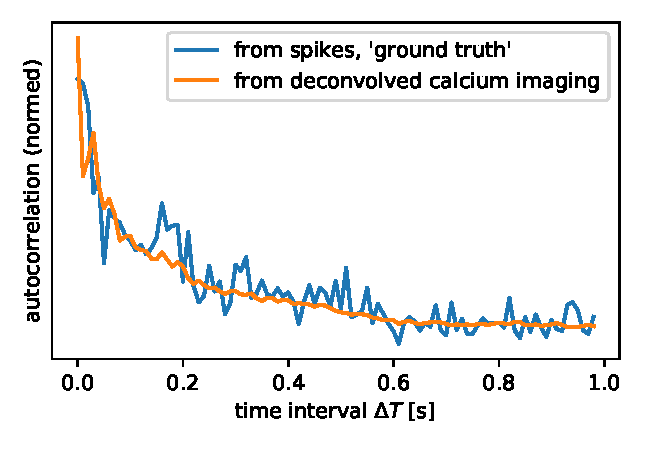
\includegraphics[width=0.5\linewidth]{./figures/comparison3_normed.pdf}
	\end{subfigure}%
	\caption{After the autocorrelation function was empirically normed, the decay obtained from the calcium trace matches nicely the ground truth. }
	\label{fig:comparison_2p_normed}
\end{figure}

I can only speculate for the reason of the large values of the autocorrelation function obtained from the calcium traces. It means that the fluorescence observations are less noisy and/or less subsampled than electrophysiological observations. Thus, either some spikes are missed by the electrode, leading to a temporal subsampled signal, or the fluorescence signal is better sampled, eventually because neurons behind the neuron of interest are also incidentally observed. 

The first hypothesis could be tested by taking the raw data from the electrodes, and averaging the data centered at spikes detected only by the calcium signal and not the electrode. If some spikes were lost in the noise, the averaging should reveal them.

The second hypothesis could be investigated by taking the raw video of the calcium fluorescence and reducing the size of the region of interest (ROI) that is used to estimate the fluorescence trace of the neuron. If it is contaminated by neurons behind, this should reduce the impact.

\section{Further analysis (Adam Packer's recording)}

The overarching goal is to investigate the hierarchy of timescales in other species than macaques. To this end
we want to start a collaboration with the Adam Packer group from Oxford. We received a sample calcium imaging recording of spontaneous activity from the somatosensory cortex of a mouse. The indicator used was GCaMP6s. 

I used the Suite2P toolbox \cite{pachitariu_suite2p:_2017} to register the frames, extract ROIs, subtract neuropil contamination and deconvolve the signal with the OASIS algorithm. I left all the parameters to their default values except the decay time of the indicator which I set as before to \SI{1.5}{s}. This yielded deconvolved calcium traces of 404 neurons with a length of 10 minutes. The autocorrelation function was calculated as before as the average of the individual autocorrelation functions.

\begin{figure}
	\begin{subfigure}{.5\textwidth}
		\centering
		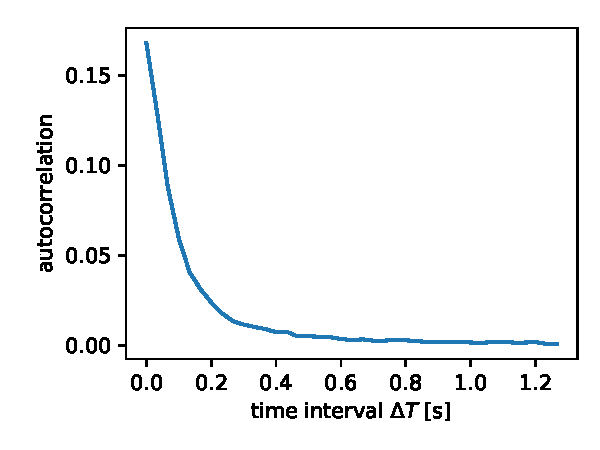
\includegraphics[width=1\linewidth]{./figures/packer_example_lin.pdf}
	\end{subfigure}%
	\begin{subfigure}{.5\textwidth}
		\centering
		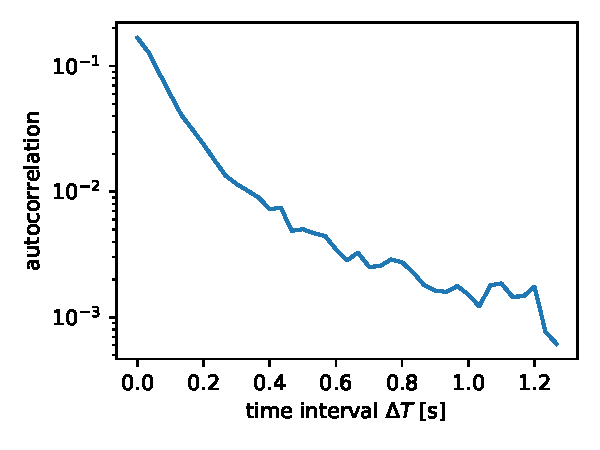
\includegraphics[width=1\linewidth]{./figures/packer_example_log.pdf}
	\end{subfigure}%
	
	\caption{Autocorrelation functions of spontaneous activity in the somatosensory cortex of a mouse, data obtained from Adam Packer.}
	\label{fig:packer_example}
\end{figure} 

The decay of the resulting autocorrelation function has a time constant of about \SI{200}{ms} (Fig.~\ref{fig:packer_example}) which is consistent with the results from macaques. Plotting the decay in a logarithmic plot, one remarks that the decay is not constant, but faster for small time intervals. This could have physiological causes (network effects, synaptic time constants), arise from averaging autocorrelation functions with different time constants  or still be an artifact of the calcium deconvolution. But nevertheless, the deconvolution approach seems to yield relatively consistent results.

A first analysis was to estimate the timescale of the 404 individual neurons and investigate whether there exist a dependence between neighboring neurons or on the position in the tissue. I therefore plotted the estimated intrinsic timescale as function of the position, but no structure is apparent (Fig. \ref{fig:packer_map_taus}).

\begin{figure}

	\centering
	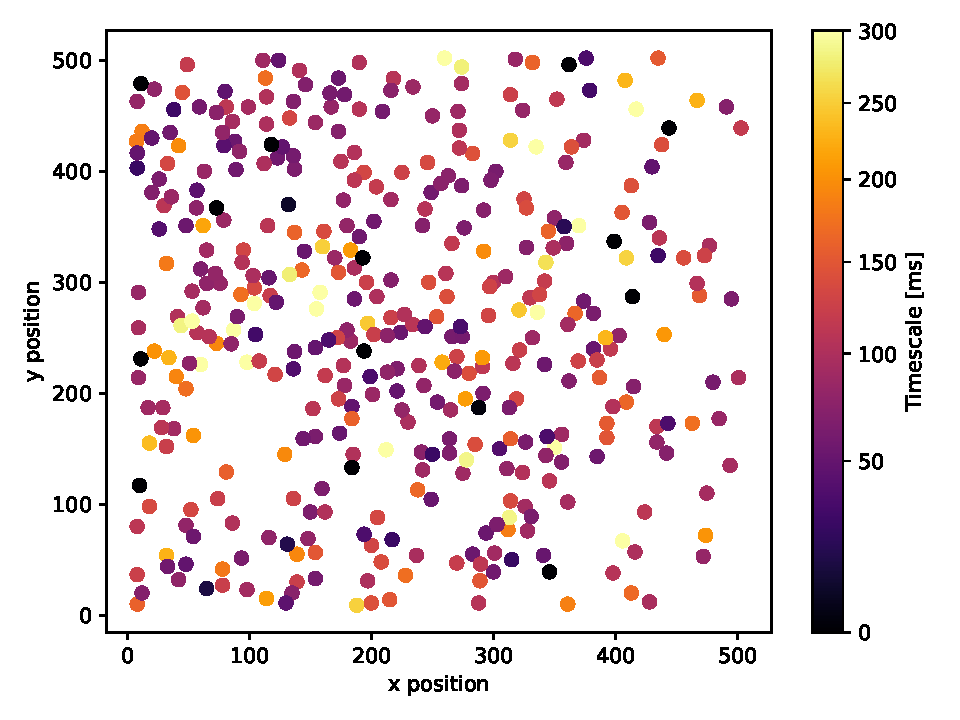
\includegraphics[width=0.85\linewidth]{./figures/map_taus.pdf}
	
	\caption{The estimated timescale of individual neurons, mapped onto the position in the field of view. One doesn't observe a structure.}
	\label{fig:packer_map_taus}
\end{figure} 


\section{Future directions}

To understand better this method, there are several further directions which would be in my view fruitful to investigate. A first step would be to analyse the original data from Theis et al. and Chen et al. and don't use the preprocessed from the spikefinder challenge. This should remove the oscillations in the autocorrelation function and eventually other biases.

In a second step, on would investigate the robustness of the results depending on the hyperparameters of the analysis, on the chosen decay time of the indicator for example. 
Then one could also look at the other open datasets where other indicators were used instead of GCaMP6s. Another nagging question is the reason for the larger amplitude of the autocorrelation obtained from calcium imaging. The difference is astonishingly large and thus important to address.

Lastly, one could search for a more direct method the calculate the timescales. The assumption of the OASIS algorithm is that in a first approximation the dynamics of the calcium fluorescence follow an AR(1) process with the input given by the spikes. As our assumption is that the network dynamics also follow an AR(1) process, one could perhaps estimate the parameters of these two overlapping process in a combined manner. 

\printbibliography

\end{document}
